\documentclass[12pt,a4paper,numbers=noenddot]{scrartcl}
\usepackage[utf8]{inputenc}
\usepackage[T1]{fontenc}
\usepackage[english]{babel}
\usepackage[pdftex]{graphicx}
\newcommand{\changefont}[3]{\fontfamily{#1} \fontseries{#2} \fontshape{#3} \selectfont}

%use autoref
\usepackage[hyphens]{url}
\usepackage{hyperref}

\usepackage{latexsym}
\usepackage{amsmath,amssymb,amsthm}

%%bib stuff
\usepackage{csquotes}
\usepackage[style=ieee]{biblatex}
\addbibresource{bib.bib}

%%%%%%extra stuff%%%%%%%%%
\usepackage{tikz}
\usepackage{tikzscale}
\usepackage{pgfplots}
\usetikzlibrary{arrows.meta}
\usetikzlibrary{plotmarks}
\usetikzlibrary{matrix}
\pgfplotsset{compat=1.5.1}
\usepackage[list=false]{subcaption}
\usepackage[export]{adjustbox}
\usetikzlibrary{positioning}
\usetikzlibrary{positioning,fit,backgrounds,arrows,shapes,automata,petri,calc,bending}
\usepackage{tabularx}
\usepackage{xtab}
\usepackage{pgfgantt}

%paragraphs
\newcommand{\properparagraph}[1]{\paragraph{#1}\mbox{}\\}
\usepackage[parfill]{parskip}

%floats
\usepackage{float}

%set margins
\usepackage[left=2cm, right=1.5cm]{geometry}

%remove section numbering
\renewcommand{\thesection}{SECTION~\Roman{section}}
%\renewcommand*{\sectionformat}{}
%\renewcommand*{\subsectionformat}{}
\renewcommand{\thesubsection}{\Alph{subsection}}
\renewcommand*{\subsubsectionformat}{}

%section heading in serif
\addtokomafont{disposition}{\rmfamily}

%set spacing to 1.5
\usepackage[onehalfspacing]{setspace}

%more space in toc for "SECTION"
\usepackage{tocloft}
\addtolength{\cftsecnumwidth}{75pt}
\addtolength{\cftsubsecnumwidth}{0pt}
\makeatletter
\renewcommand{\@cftmaketoctitle}{}
\makeatother


\usepackage{lipsum}

%page x of y
\usepackage{lastpage}
\usepackage{fancyhdr}
\pagestyle{fancy} 
\cfoot{Page \thepage\ of \pageref{LastPage}}

\begin{document}
\pagestyle{empty}
  \begin{titlepage}
$
\begin{array}{l}
\resizebox{3cm}{!}{\includegraphics{ee_logoV2.tikz}}
\end{array}
$ {\Large \changefont{pag}{m}{n}Engineering --- Consulting --- Design}

  	\vspace*{3cm} 
  	
  	\begin{center} \large 
  		Project Report
  		\vspace*{2cm}
  		
  		{\huge Biosynthetic Fuel}
  		\vspace*{\fill}
  		
  		\textbf{06/25/2019}

  		\vspace*{1.5cm}
  		
  		Karlsruhe Institut of Technology - English for Engineers
  	\end{center}
  \end{titlepage}
\setcounter{page}{1}

\section{The Project Statement}
\section{The Executive Summary}
\newpage
\section{Table of Contents}
\tableofcontents
\newpage
\section{The Working Papers}
\subsection{Synfuels}
\tablehead{
	\hline
	\textbf{HEADING} & \textbf{ANALYSIS/DISCUSSION} & \textbf{REFERENCES} \\
	\hline
}
\tabletail{\hline \multicolumn{3}{|r|}{\footnotesize continued on next page} \\ \hline}
\begin{xtabular}{|p{3.8cm}|p{8.3cm}|p{4.2cm}|}
	\vspace*{-1.25\baselineskip}\subsubsection{Topic Title}
	& 

	& 
	\\
	\vspace*{-1.25\baselineskip}\subsubsection{Findings}
	& 

	&
	\\
	\vspace*{-1.25\baselineskip}\subsubsection{Problems encountered}
	& 

	&
	\\
	\vspace*{-1.25\baselineskip}\subsubsection{Solutions}
	& 

	&
	\\
	\vspace*{-1.25\baselineskip}\subsubsection{Current Developments}
	& 
	
	&
	\\
	\vspace*{-1.25\baselineskip}\subsubsection{Conclusion}
	& 
	
	&
	\\
	\vspace*{-1.25\baselineskip}\subsubsection{Personal Comments}
	& 
	
	&
	\\
	\hline
\end{xtabular}

\newpage
\subsection{Syngas}
\begin{xtabular}{|p{3.8cm}|p{8.3cm}|p{4.2cm}|}
	\vspace*{-1.25\baselineskip}\subsubsection{Topic Title}
	& 
	
	& 
	\\
	\vspace*{-1.25\baselineskip}\subsubsection{Findings}
	& 
	
	&
	\\
	\vspace*{-1.25\baselineskip}\subsubsection{Problems encountered}
	& 
	
	&
	\\
	\vspace*{-1.25\baselineskip}\subsubsection{Solutions}
	& 
	
	&
	\\
	\vspace*{-1.25\baselineskip}\subsubsection{Current Developments}
	& 
	
	&
	\\
	\vspace*{-1.25\baselineskip}\subsubsection{Conclusion}
	& 
	
	&
	\\
	\vspace*{-1.25\baselineskip}\subsubsection{Personal Comments}
	& 
	
	&
	\\
	\hline
\end{xtabular}

\newpage
\subsection{Engine Modifications}
\begin{xtabular}{|p{3.8cm}|p{8.3cm}|p{4.2cm}|}
	\vspace*{-1.25\baselineskip}\subsubsection{Topic Title}
	& 
	
	& 
	\\
	\vspace*{-1.25\baselineskip}\subsubsection{Findings}
	& 
	
	&
	\\
	\vspace*{-1.25\baselineskip}\subsubsection{Problems encountered}
	& 
	
	&
	\\
	\vspace*{-1.25\baselineskip}\subsubsection{Solutions}
	& 
	
	&
	\\
	\vspace*{-1.25\baselineskip}\subsubsection{Current Developments}
	& 
	
	&
	\\
	\vspace*{-1.25\baselineskip}\subsubsection{Conclusion}
	& 
	
	&
	\\
	\vspace*{-1.25\baselineskip}\subsubsection{Personal Comments}
	& 
	
	&
	\\
	\hline
\end{xtabular}

\newpage
\subsection{Engine Control (Marvin)}
\begin{xtabular}{|p{3.8cm}|p{8.3cm}|p{4.2cm}|}
	%heading
	\vspace*{-1.25\baselineskip}
	\subsubsection{Introduction}
	&
	%main
	The engine control is a vital component of an internal combustion engine (IEC). Today the control of engines in small engines found in cars and trucks is done electrically with a so called \textit{engine control unit} (ECU).
	
	The ECU handles multiple control loops with each fulfilling a specific task. For example:
	& 
	%ref
	\fullcite{kiencke2005}
	\\
	%heading
	&
	%main
	\begin{itemize}
		\item \textbf{Lambda Control}: Controls air/fuel mixture
		\item \textbf{Idle Speed Control}: Keeps the idle speed constant
		\item \textbf{Knock Control}: Prevents knocking
		\item \textbf{Cylinder Balancing}: Ensures smooth running of the engine
	\end{itemize}
	&
	%ref
	\\
	%heading
	\vspace*{-1.25\baselineskip}
	\subsubsection{Findings}
	&
	%main
	For many years, the requirements for an ECU have been pretty much the same. The ECU just had to perform the tasks listed above reliably. Parameters of the engine with its peripherals (which form a dynamic system in sense of control engineering) were constant, i.e. they were assumed to stay at a constant value over time. 
	&
	%ref
	
	\\
	%heading
	Lambda Control
	&
	%main
	On main ECU task is lambda control. With the AFR (air-fuel ratio) controller, the injection of fuel is controlled such that the fuel is burned completely. This helps conserving fuel and is necessary for the so called catalytic converter, which clears the exhaust gases from many pollutants.
	
	This process is illustrated by the following block diagram:
	&
	%ref
	
	\\
	%heading

	&
	%main
	{
		\center
		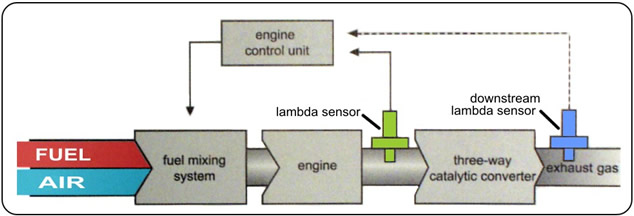
\includegraphics[width=8cm]{material/marvin/LambdaFunctionalDiagram.jpg}
	}
	&
	%ref
	\url{secure.lambdapower.co.uk}
	\\
	%heading
	(Idle) speed control
	&
	%main
	If the car is in neutral, that is no gear is engaged, a constant engine speed (the idle speed) is desired. This is necessary to keep the motor running and to drive auxiliary devices (air conditioning, power steering, ...) In the most cases it is sufficient to control the speed in a quite large band, i.e. in a way that the engine doesn't stall (lower boundary) but doesn't run to fast to conserve fuel and to save the environment (upper boundary).
	
	Constant load situations is another state which should be considered when designing a engine speed controller. Constant load occurs e.g. when driving (without accelerating) on a long flat highway or pulling a trailer up a hill with constant speed. In either case, small speed deviations are tolerable from a technical standpoint.
	&
	%ref
	\fullcite{Subramanian2018}
	\\
	%heading
	\vspace*{-1.25\baselineskip}
	\subsubsection{Problems encountered}
	&
	%main
	In recent years, customers begun to require higher levels of comfort when driving a car or truck. They expect a continual smooth ride regardless of the fuel used and of the usage of additional car accessories.
	&
	%ref
	
	\\
	%heading
	From a consumer point of view
	&
	%main
	Especially modern air conditioning or infotainment systems require much electrical power. To generate the power consumed by these devices, the engine has to drive an alternator. Because these systems can be switched on or off rapidly, they introduce high frequency disturbances to the engine load which the ECU has to remedy. A sophisticated control structure is required in order to prevent high fluctuations of the engine speed which can cause noticeable depreciations of ride smoothness.
	
	Today fossil fuels become more expensive which causes customers to consider fuel ratings when buying a new car. But also the majority of the customers don't want to get to technical with the car. A simple gas stop should be enough.
	&
	%ref
	
	\\
	%heading
	From an environmental point of view
	&
	%main
	In the past, when designing an ECU for an \textsc{Otto} or \textsc{Diesel} engine, the engineer mostly knew what to expect. E.g. gas refined in refineries has very similar properties around the world. Because of that, characteristic curves could be linearized around some operating point. This simplifies analysis and synthesis of control systems dramatically but is only allowed, when the deviations from the operating point are small. If these deviations are large or the operating point is not constant, these simplifications are no more valid and non linear models have to be used.
	
	But to acquire these models, some parameters of the fuel have to be measured (these could include the octane number in the case of gas or the cetan number in the case of diesel). Since it is expensive to measure them and not reasonable to determine them online in the car, they have to be estimated in real time.
	
	This step is rather challenging but vital to ensure emissions complying with the law and to achieve high fuel efficiency ratings.
	&
	%ref
	\\
	%heading
	From the manufactures point of view
	&
	%main
	For the manufacturer it is rather risky to focus on one bio fuel solution at the moment. The car market is volatile and innovations can become successful or die rather quickly. From an engineering and economical perspective, a new ECU should be easily adaptable to different fuel types and optimally completely different technologies.
	&
	%ref
	
	\\
	\vspace*{-1.25\baselineskip}\subsubsection{Solutions}
	& 
	Ideally an ECU lineup would offer an ECU for 'liquid fuel for gas engines' which then automatically adapts to the type of fuel present in the gas tank, without the user noticing.
	&
	\\
	\vspace*{-1.25\baselineskip}\subsubsection{Current Developments}
	& 
	Modern approaches like cascading control or prediction of system states with \textsc{Kalman} filtering could be useful tools when designing a controller.
	&
	\url{https://www.controleng.com/articles/fundamentals-of-cascade-control/}
	\url{http://web.mit.edu/kirtley/kirtley/binlustuff/literature/control/Kalman%20filter.pdf}
	\\
	\vspace*{-1.25\baselineskip}\subsubsection{Conclusion}
	& 
	New ECUs should adapt more modern approaches in control design to allow the usage of new bio fuels.
	&
	\\
	\vspace*{-1.25\baselineskip}\subsubsection{Personal Comments}
	& 
	Research engine control fundamentals specific to new (synthetic) fuels is a quite hard task. Compared to the about 100 years of automobile history, fuels other than gas or diesel are rather new areas of wide scientific interest. Furthermore the development of ECUs in hard- and software is a labour intensive progress mostly done by private companies, which leads to sparse public available information about their inner workings.
	&
	\url{www.bosch-mobility-solutions.com/en/products-and-services/commercial-vehicles/powertrain-systems/natural-gas/electronic-engine-control-unit/}
	\\
	\hline
\end{xtabular}

\newpage
\section{Analysis Summaries}
\newpage
\section{Resources}
\newpage
\section{Glossary}
\begin{tabularx}{\textwidth}{p{3cm} l}
	IEC & Internal Combustion Engine \\
	ECU & Engine Control Unit \\
\end{tabularx}	
\newpage
\section{Evaluations}
\newpage
\section{Reference List}
\printbibliography
\newpage
\section{Other}

\subsection{Project Progress}
\begin{ganttchart}{1}{28}
	\gantttitle{CW 26 (June)}{7} \gantttitle{CW 27 (July)}{7} \gantttitle{CW 28 (July)}{7} \gantttitle{CW 29 (July)}{7} \\
	\gantttitlelist{24,...,30}{1} \gantttitlelist{1,...,7}{1} \gantttitlelist{8,...,14}{1} \gantttitlelist{15,...,21}{1} \\
	\ganttgroup{Project Paper}{1}{20} \\
	\ganttbar[bar/.append style={fill=blue}]{WP: synfuel}{1}{2} \\
	\ganttbar[bar/.append style={fill=red}]{WP: syngas}{3}{7} \\
	\ganttmilestone{Finalize Paper}{22} \\
	
	\ganttgroup{Presentation}{14}{20} \\
	\ganttbar[bar/.append style={fill=green}]{Task 1}{1}{2} \\
	\ganttbar[bar/.append style={fill=yellow}]{Task 2}{3}{7} \\
	\ganttmilestone{Finalize ppt}{22} \\
	
	\ganttmilestone{Project Due}{24}
	\ganttlink{elem3}{elem8}
	\ganttlink{elem7}{elem8}
\end{ganttchart}

\end{document}